%%%%%%%%%%%%%%%%%%%%%%%%%%%%%%%%%%%%%%%%%%%%%%%%%%%%%%%%%%%%%%%%%%%%%%%%%%%%%
%%% PIA Tutorial
%%% Julian Uszkoreit
%%% julian.uszkoreit@rub.de
%%%%%%%%%%%%%%%%%%%%%%%%%%%%%%%%%%%%%%%%%%%%%%%%%%%%%%%%%%%%%%%%%%%%%%%%%%%%%

\pdfminorversion=4
\documentclass[a4paper,11pt,twoside]{article}
\usepackage[T1]{fontenc}
\usepackage[utf8]{inputenc}
\usepackage[onehalfspacing]{setspace}
\usepackage{changepage}
\usepackage{emptypage}
\usepackage{listingsutf8}
\usepackage{graphicx}
\usepackage[dvipsnames]{xcolor}
\usepackage[small,bf,margin=1cm,singlelinecheck=true]{caption}
\usepackage[a4paper]{geometry}
\usepackage{layout}
\usepackage{hyperref}
\usepackage[ddmmyyyy,hhmmss]{datetime}

% set font family
\usepackage{lmodern}
\sffamily %to load T1lmss.fd

% Load 'sans small caps' from helvet:
\usepackage{helvet}
\sffamily %to load T1phvss.fd
% Substitute non-existing lmss/bx/sc with phv/bx/sc
\DeclareFontShape{T1}{lmss}{bx}{sc} { <-> ssub * phv/bx/sc }{}
% Can also pick the sans small caps:
\DeclareFontShape{T1}{lmss}{m}{sc} { <-> ssub * phv/m/sc }{}

\renewcommand*\rmdefault{lmss}

% to nicely show menu entries
\newcommand{\menu}[1]{{\scshape\bfseries #1}}
% to nicely show files
\newcommand{\filepath}[1]{{\scshape\bfseries #1}}
% to nicely show kniem nodes
\newcommand{\knimenode}[1]{{\scshape\bfseries #1}}


\title{Tutorial of PIA -- Protein Inference Algorithms}
\author{Medical Bioinformatics\\
	Medizinisches Proteom-Center\\
	Ruhr-Universität Bochum}


\begin{document}

%%%%%%%%%%%%%%%%%%%%%%%%%%%%%%%%%%%%%%%%%%%%%%%%%%%%%%%%%%%%%%%%%%%%%%%%%%%%
%%% TITLE PAGE
\thispagestyle{empty}
\begin{titlepage}
	\vspace*{\fill}
	\begin{adjustwidth}{-2cm}{-2cm}
		\begin{center}
			{\huge \textbf{PIA -- Protein Inference Algorithms\\
					Tutorial}\\[2cm]}
		\end{center}
	\end{adjustwidth}

	\begin{center}
		
\includegraphics[width=0.5\textwidth]{graphics/pia_logo_big}\\[2cm]

		{\large Medical Bioinformatics\\
			Medizinisches Proteom-Center\\
			Ruhr-Universität Bochum\\[0.5cm]}
		{\large https://github.com/mpc-bioinformatics/pia\\[0.1cm]}
	\end{center}

	\vspace*{2cm}
	\begin{center}
		Version \today{}, \currenttime{}.
	\end{center}
	\vspace*{\fill}
\end{titlepage}

%%%%%%%%%%%%%%%%%%%%%%%%%%%%%%%%%%%%%%%%%%%%%%%%%%%%%%%%%%%%%%%%%%%%%%%%%%%%

\tableofcontents
\newpage


\section{Introduction}

\subsection{PIA -- Protein Inference algorithms}

PIA is an open source toolbox for MS based protein inference and identification
analysis. As in bottom-up MS proteomics actually peptides are identified, but
most often the entities of interest are proteins, the protein content of an
analysed sample must be constructed from the knowledge of the contained
peptides. This step is known as "protein inference" and is the heart of PIA.
Furthermore, PIA can be used to inspect, analyse, perform quality checks
on and filter identified peptide spectrum matches (PSMs) and peptides. This can
be performed either via a web frontend, KNIME nodes or the command line. While
the latter method is intended for advanced scripting and the command line can
now also be downloaded as a Docker image, we will mainly discuss the usage of
KNIME nodes in this tutorial.


\subsection{Prerequisites}

All data and workflows can be downloaded in the tutorial repository at
\url{https://github.com/julianu/pia-tutorial}.

\begin{itemize}
	\item Knowledge of mass spectrometry based bottom-up peptide identification
	\item Basic knowledge of KNIME and constructing workflows with KNIME
	\item You should be familiar with the OpenMS spectrum identification using
	KNIME (if not, please refer to the OpenMS tutorials at
	\url{http://www.openms.de/tutorials/})
	\item The tutorial was tested using the stable OpenMS 2.1.0 nodes and KNIME
	3.3.1
	\item For parts of the tutorial you need the R nodes of KNIME
\end{itemize}

\subsection{Version}

This tutorial was created on \today{} at \currenttime{}.


\newpage
\section{Installation of PIA KNIME nodes}

If not yet done, you first need to download and install KNIME to your system
(\url{https://www.knime.org/downloads/overview}). The easiest way to work with
PIA inside KNIME is to install the "\textbf{KNIME Analytics Platform + all free
extensions}", which comes with many nice nodes and functions, including the PIA
nodes.

If you did install KNIME without all free extensions, or upgraded from an older
version, you can install the nodes from the community contributions repository.
For this start KNIME and go to \menu{Help > Install New Software...}. Select the
community contributions repository under the \menu{Work with} drop down menu, it
should have th eaddress
\url{http://update.knime.org/community-contributions/trusted/3.3}. The PIA nodes
can be found in the \menu{Bioinformatics \& NGS} group or simply by searching
for them. Select the PIA nodes, click next, accept the license and restart KNIME
after the installation is finished.

If all went well, you will see the PIA octopus on the splash screen of KNIME
(together with all the other icons) and you will find the PIA nodes inside the
\menu{Community Nodes} in the Node Repository (usually left bottom side of
screen). This tutorial also needs the OpenMS and R nodes to be
installed. These need to be installed manually as well, if you did not install
the "KNIME Analytics Platform + all free extensions" as recommended above. You
should also already be familiar with the OpenMS spectrum identification using
KNIME.


\newpage
\section{Running PIA in KNIME}

First download the workflows and data for the tutorial at
\url{https://github.com/julianu/pia-tutorial}.


\subsection{First workflow}

First, we will run a minimal workflow identifying spectra in a mzML file with
the search engine X!Tandem and using PIA for the protein inference and also
analysis of the identified PSMs and peptides.

Import and open the workflow \filepath{PIA\_first\_analysis} from the provided
workflows into your KNIME workspace. Please select the file
\filepath{lfq\_spikein\_dilution\_1.mzML} as the analysed mzML file (upper
\knimenode{Input File}) and the FASTA file \\
\filepath{s\_pyo\_sf370\_potato\_human\_target\_decoy\_with\_contaminants.fasta}
as \\ database for spectrum identification. We used X!Tandem for spectrum
identification in this workflow. If you like, you can change it to any other
supported software in KNIME, the basic configuration settings are:

\begin{itemize}
	\item 10 ppm precursor tolerance
	\item 0.4 Da fragment tolerance
	\item tryptic digestion with up to 2 missed cleavages
	\item fixed Carbamidomethyl of C and variable Oxidation of M
\end{itemize}

The \knimenode{PeptideIndexer} is needed to add the protein / accession
information to the identified peptide spectrum matches (PSMs). For the tutorial
data, use "REV\_" as the decoy string and prefix as decoy position and make sure
that Trypsin is set as enzyme with none as specificity. After adjusting the
\knimenode{Input File} nodes (and maybe the search node), run the workflow until
the \knimenode{PIA Compiler}.

This node takes a list of files. Note, that the ports from OpenMS
need to be converted into a URI file list. You could alternatively use a
\knimenode{List Files} node to select the files containing prior performed
spectrum identifications in any supported format like Mascot Dat, X!Tandem's
XML files, Proteome Discoverer's MSF files or any mzIdentML file, and use these
files as input for the compiler. This node is necessary to structure the data
before a PIA analysis. It must be performed only once per set of identification
files. The \knimenode{PIA Compiler} has as input settings only a compilation
name, which can be chosen freely. The number of files passed to PIA is not
limited, though processing more files needs more main memory. Each file in the
compilation gets a FileID, which you can explore with some additional
information of the merge looking at the \menu{View: summary} after runing the
\knimenode{PIA Compiler}. These IDs can also be used for filtering and advanced
settings later on.

\begin{figure}[ht!]
	\centering
	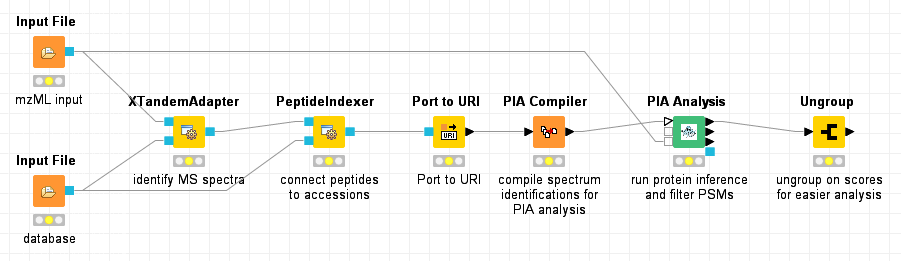
\includegraphics[width=0.8\textwidth]{graphics/first_analysis_workflow}
	\caption{A small protein analysis workflow using X!Tandem for spectrum
	identification and PIA for protein inference.}
\end{figure}

The first connected port is for the PIA compilation, directly coming from the
compiler node. If you should have a saved compilation, you could also use this
and  the second input port. The first port with a suitable configured file will
be processed. The third input port is used to pass spectrum data to PIA, which
can later be used to visualise automatically annotated spectra. If you don't
want to use the spectrum viewer, you should not connect anything to this port,
as the matching of the PSMs to their spectra might take some time.


\subsubsection{General Settings}

After running the compiler, open the settings of the \knimenode{PIA Analysis}
node. You will find four tabs for the settings: one general and one for each of
the levels of analysis (i.e. PSMs, peptides and proteins). If you connected the
compiler node directly to the analysis node, select the column containing the
PIA XML file (there should mostly be only one named "gzipped PIA XML file").
You can also set, whether PIA should fail if no decoys were found in the
analysis, whether PSM sets should be created and whether modifications should
be considered to distinguish peptides (see Figure \ref{pia_settings_general}).
Creating PSM sets should always be used, if the same spectrum file was analysed
with different search engines. This option will then combine the results of
multiple searches, otherwise it can be deselected. Mostly, a peptide and it's
scoring influence for the proteins should only be described by its sequence. If
you have stable modifications, though, you can select to distinguish peptides
by sequences and modifications. The \knimenode{PIA Analysis} node allows to
export the analysis into several file formats. The level of the export (PSM,
peptides and protein) as well as the format can be selected appropriately.

\begin{figure}[ht!]
	\centering
	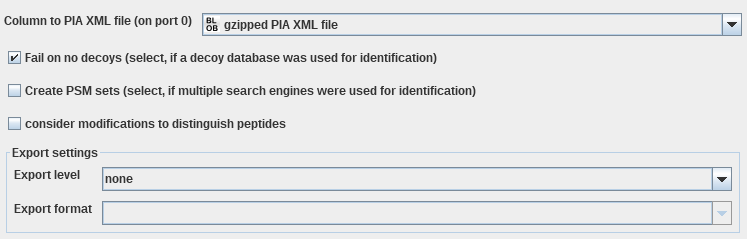
\includegraphics[width=0.9\textwidth]{graphics/pia_settings_general}
	\caption{The general settings dialog of the \knimenode{PIA Analysis} node.}
	\label{pia_settings_general}
\end{figure}


The analyses at the PSM and peptide level of PIA will be performed only for the
input file given by the FileID in the respective settings tab. Usually, the IDs
start with 1 and are sorted by the order of the given input files. A special
case is the combination of all runs (either with PSM sets or without), also
called overview, which always has the ID 0. The 0 for FileID is the default for
the PSM and peptide level analyses.


\subsubsection{PSM Settings}

Now, have a look at the PSMs settings of the \knimenode{PIA Analysis}. The
first setting is the just mentioned file ID, which is 0 in the example and thus
reflects the combination of all results (Note: we have only one file in the
example, but the "Combined FDRScore" will only be calculated on file 0. For one
single input file, though, it is identical to the normal FDRScore). Next you
can choose to calculate the false discovery rate (FDR), and thus also FDRScore
and q-value, for all input files. The FDRScore \cite{jones2009} smoothes the
FDR q-values in an analysis and thus facilitates a better discrimination of
identifications instead of using the FDR q-values alone. If PSM sets will be
created, also the Combined FDRScore can be calculated, which furthermore allows
the combination of search results from multiple MS runs as well as
identifications from different search engines.

\begin{figure}[ht!]
	\centering
	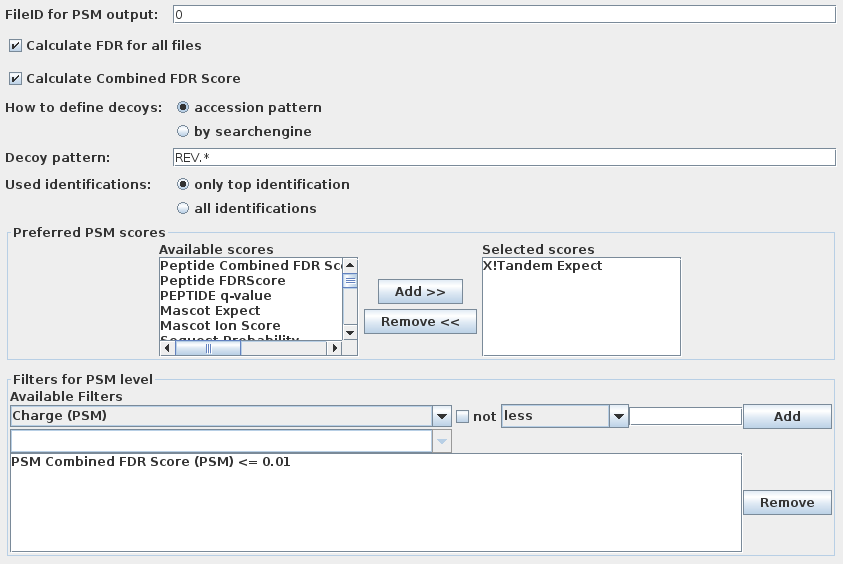
\includegraphics[width=0.9\textwidth]{graphics/pia_settings_psms}
	\caption{The PSMs settings dialog of the \knimenode{PIA Analysis} node.}
	\label{pia_settings_psms}
\end{figure}

A very important step is the selection of how decoys are distinguished from
target identifications. PIA allows to use regular expressions for this, which
are applied to the accessions. In the example in Figure
\ref{pia_settings_psms}, "REV.*" is set as regular expression. So each
accession starting with the string "REV" (and all its peptides) will be
assigned to be decoys and all not matching accessions to be targets.
Alternatively, if "by search engine" is selected, identifications must be
annotated in the input files as targets and decoys. This is e.g. the case if in
Mascot the "Decoy" option is selected for an MS/MS search. For better
compatibility though, the usage of a target-decoy database and the assignment
by regular expressions is recommended.

Some search engines report more than one identification per spectrum. In the
next option, you can choose to either use all these identifications or only the
one with the best score for FDR analysis and all following steps. Finally, you
can select which scores are used for FDR estimation. If a search engine reports
multiple score (e.g. X!Tandem's Hyperscore and Expect), you can choose the
preferred score here. If no score was chosen, PIA will use the main score of
the search engine (or, if this was not given, just any score).

All the settings up to this point are used for the FDR calculation (except for
the output file ID) and influence the peptide and protein reports as well. The
filters afflict only the PSM level and its report. Here you can chose from the
available filters and set the parameters accordingly. For score filters it is
necessary to select the according score as well (below the filters selection).
After selecting a filter and setting the parameters, don't forget to click
\menu{Add}. The currently activated filters will be shown in the list. In the
example workflow, a filter for the "Combined FDRScore <= 0.01" is selected.
Keep in mind, that all filters have to be fulfilled for a PSM to pass the
filters.


\subsubsection{Peptides Settings}

Next, select the peptides settings. All settings here are only for the peptide
export and do not afflict the protein inference. Therefore, you can also turn
the peptide inference off and will get an empty report. This might be required,
if you need to save time and main memory during the analysis. The selection of
the file ID has the same meaning as on the PSM level (exporting only
information of this file, or 0 for the combination of all results). Also the
filters are used in the same way. An exception are the PSM level filters: with
these, the PSMs which are actually used to create peptides, are filtered. In
the example workflow and in Figure \ref{pia_settings_peptides}, only PSMs with
"Combined FDR Score <= 0.01" are inferred to peptides.

\begin{figure}[ht!]
	\centering
	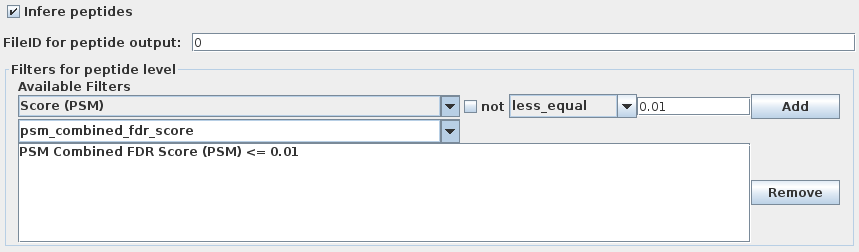
\includegraphics[width=0.9\textwidth]{graphics/pia_settings_peptides}
	\caption{The peptides settings dialog of the \knimenode{PIA Analysis} node.}
	\label{pia_settings_peptides}
\end{figure}


\subsubsection{Protein Inference and Protein Settings}

Finally, take a look at the proteins settings. Also the protein inference can
be turned off, if you are only interested in analyses on the PSM or peptide
level. First, you have to chose an inference method. PIA provides you with
three different methods (for a more thorough explanation of these methods,
please refer to \cite{uszkoreit2015})

\begin{figure}[ht!]
	\centering
	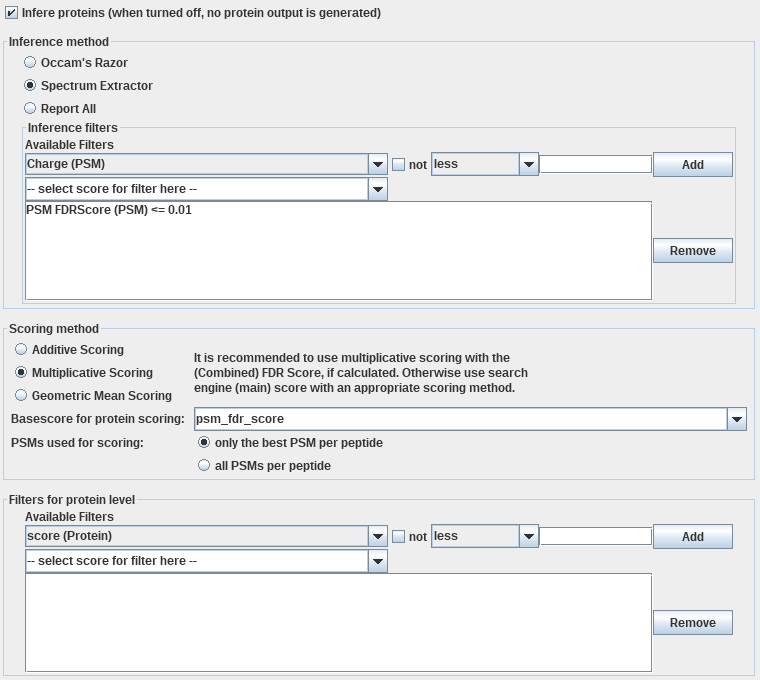
\includegraphics[width=0.9\textwidth]{graphics/pia_settings_proteins}
	\caption{The proteins settings dialog of the \knimenode{PIA Analysis} node.}
	\label{pia_settings_proteins}
\end{figure}

\begin{itemize}
	\item \textbf{Occam's Razor} is based on the parsimony principle and
	returns the smallest set of proteins, which explain all identified
	peptides. This is a very widely used strategy for protein inference.

	\item \textbf{Spectrum Extractor} is the recommended method. It is also
	based on the parsimonious approach, but assigns a spectrum to only one
	peptide. This peptide is selected in such a way, that it increases the
	score of the most probable, possible protein group.

	\item \textbf{Report All} This is actually no real inference, but reports
	all possible protein groups, based on the data. Use this with caution and
	only when you know, what you are doing!
\end{itemize}

After selecting the inference method, you can apply a variety of filters, which
should be applied on PSM, peptide and protein level and directly afflict the
results of the inference. You should almost always filter on the FDR, either
using the FDRScore or the Combined FDR Score, usually on a value of about 0.01.
But you could also set filters which make a protein to require at least two
peptides to be valid, and many more filters.

Next, you need to select the scoring method. Here, you should use "additive
scoring" only if your base score has a "higher score is better" probability,
like e.g. the Mascot Ion Score or X!Tandem's Hyperscore. Otherwise, use one of
the other two scorings. The "multiplicative scoring" takes the number of
identified peptides into account, in the way that the final protein score is
usually better with more distinct peptides. The "geometric mean scoring" on the
other hand calculates the mean of all peptide scores.

Finally, you need to select the base score and whether only the best PSM
(recommended) or all PSMs of a peptide should be used for scoring. In our
example, the Combined FDRScore is used. (Note: As base score you can only
select scores on the PSM level, as the peptides will be generated during the
inference according to your applied filters.)

The protein report can also be filtered in the same way as the PSMs and
peptides report. Be aware, that this is significantly different to setting an
inference filter on protein level: filters applied for the inference make it
possible to not even create a protein group. Filters on the protein report
afflict only what is reported.


\subsubsection{A word on filters}

Though PIA provides you with many filters on each of the PSM, peptide and
protein level, you can also apply these filters later in the workflow. For
this, you can simply apply an appropriate \knimenode{Row Filter} node after
running the \knimenode{PIA Analysis}. But also keep in mind that setting the
inference filters on the protein level are behaving very differently, as
explained above.


\subsection{Looking at the Results}

Now run the \knimenode{PIA Analysis} node. This can, depending on the loaded
data, take some time. The example data should be processed in a few moments
though. The node has four output ports: the first two are the (filtered)
reports on the PSM and peptide level for the selected input file, the third is
the protein level report and the last is a file port for the exported data, if
any was created as set in the general settings.


\subsubsection{Analysis Viewer}

To explore the results of the analysis, right click on the \knimenode{PIA
Analysis} node after the execution finished and select the \menu{View: PIA
Results Analysis}. In the top left corner you will see all the inferred protein
groups. PIA always works with protein groups, even if such a group might
contain only one accession. All the accessions in one group have exactly the
same evidence, i.e. the same PSMs and peptides, and cannot be distinguished on
the given data and applied inference settings. The score is calculated using
the selected base-score and scoring method.  A higher score is always better
(for base scores with "lower score better" a log value is used for
transformations). If the complete protein sequences were provided, the
coverages for the proteins are calculated. Furthermore, the number of assigned
spectra, PSMs and peptides are given. If the FDR was calculated, also the decoy
status and the FDR q-value will be given.

\begin{figure}[ht!]
	\centering
	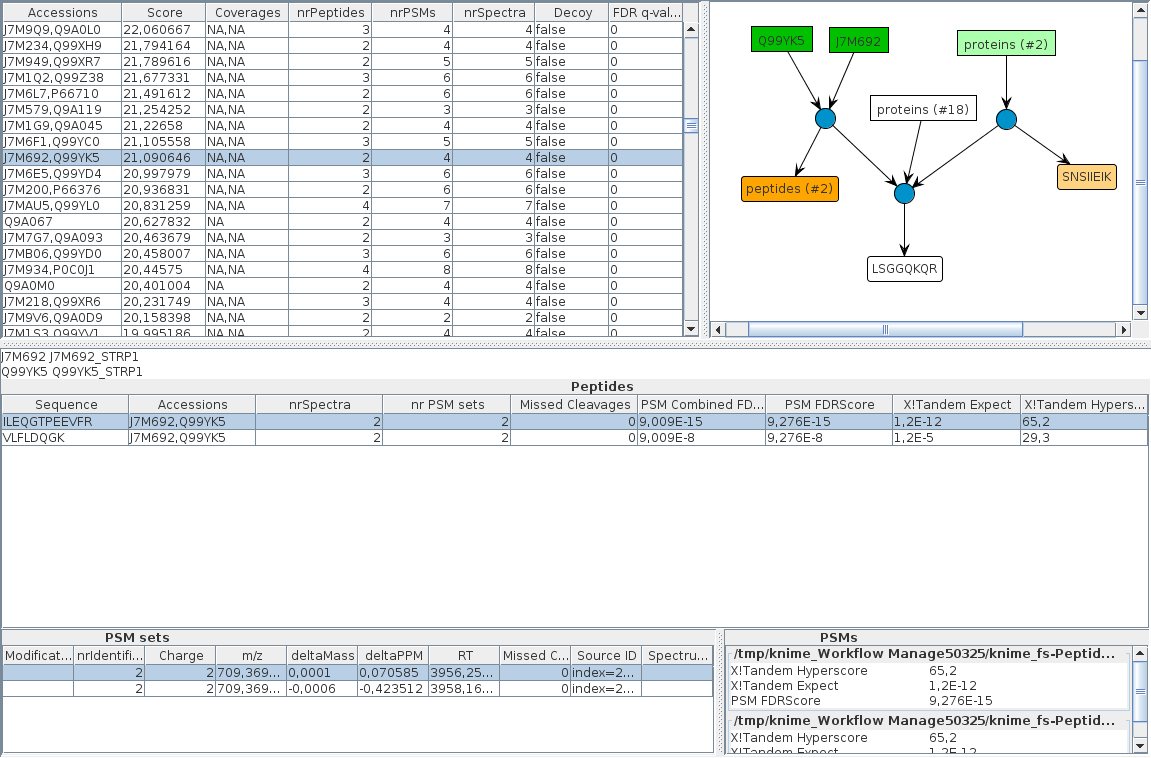
\includegraphics[width=0.9\textwidth]{graphics/screenshot_PIA_analysis}
	\caption{The PIA analysis viewer allows an intuitive exploration of the
	data.}
	\label{pia_analysis}
\end{figure}

For the currently selected protein group, the assigned (not filtered) peptides
are listed with their information in the middle of the window. On the bottom
left, all PSM sets of the selected peptide are listed and on the bottom right
finally the individual PSMs are given. If the spectrum file was given, you can
view the annotated spectrum when clicking on the button by the PSM (see also
PSM Results).

On the top right you will see a directed graph showing the relations between
accessions of the currently selected protein group and its peptides and PSMs.
In the example workflow, take a look at the groups "J7MBF9,Q99XR9" (it has
a score of 52.74) and "Q9A0M0" (score of 20.40). The accessions of the selected
group are coloured in dark green. Accessions of (not reported) sub-groups are
given in light-green without border and accessions reported in other groups in
light green with black border. Peptides are coloured in orange (dark for the
selected group, light for other groups in the same way as accessions). The blue
circles are drawn only to construct a correct tree. Nodes which hold multiple
items, can be expanded by double clicking on them, as can peptides to show their
PSMs. All items can be re-arranged by drag-and-drop.


\subsubsection{PSM Results}

To look at the PSM level report, right click on the node and select \menu{0:
PSM results}. in this table you have almost all available information for the
PSMs, like the amino acid sequence, a list of accessions, modifications,
precursor charge, m/z value, the mass error, etc. Also, you have three columns
for the scores (scores, score names and score shorts), which are lists each.
Here, the score on a given position in the list corresponds to the score name
and its short (which is an abbreviated name) on the same positions in the list.
This makes it possible to export multiple scores in one row. In our example, we
have only the Combined FDR score, though.

For easier analysis, the scores can be ungrouped using the \knimenode{Ungroup}
node on the PSM report, which is the last step in the workflow. Take a quick
look at the \knimenode{Ungroup}'s settings and verify, that it is set to
ungroup on the three score columns (and not the accessions). Run the node and
look at the results: the score columns contain now individual names and
numbers, which can be used for further sorting and filtering.

An alternative way to look at all reported PSMs (and not the sets) is using the
"PSM Spectrum Viewer". Here you can see the PSMs together with the
automatically annotated spectra (using \cite{perez2015}). This only works, if
you connected the identified spectrum file to the third PIA input port.

\begin{figure}[ht!]
	\centering
	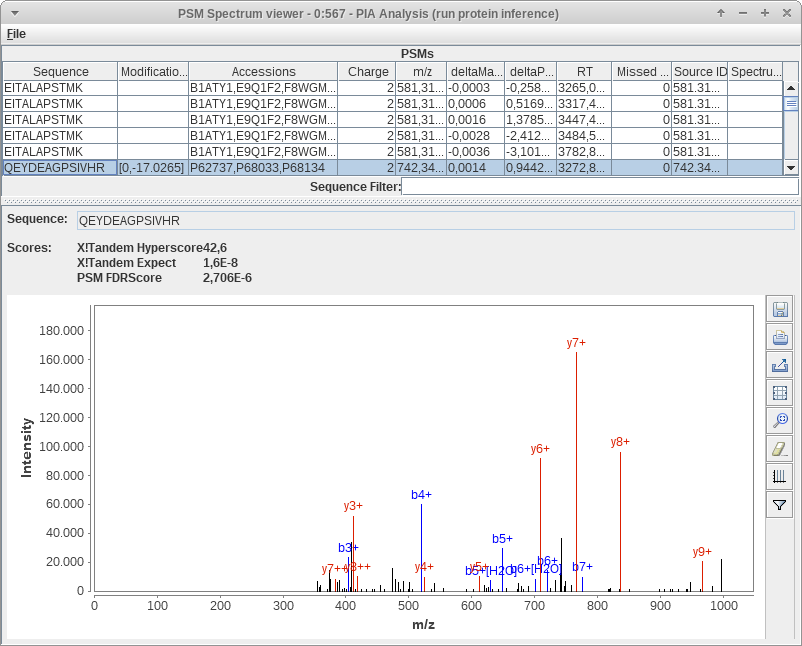
\includegraphics[width=0.9\textwidth]{graphics/screenshot_PSM_spectrum_viewer}
	\caption{The PSM spectrum viewer showing an automatically annotated
	spectrum.}
	\label{pia_psm_spectrum_viewer}
\end{figure}


\subsubsection{Peptide Results}

The peptide results are given in the same way as the PSM results. The peptides
are inferred either with or without taking modifications into account.


\subsubsection{Protein Results}

The created protein table on the third port holds almost the same information
as the table in the Analysis Viewer. Node, that the accessions are lists again,
as PIA always reports protein groups. Additionally, each group has a clusterID,
which represents the connected set or tree in the PIA intermediate structure.
Elements in such a cluster are connected by their relations of accessions and
PSMs, as can be seen in the Analysis Viewer on the top right. This does not
mean, that reported protein groups with the same cluster ID share a peptide,
but they are in the same component (a tree in the top right region of the
\menu{Analysis Viewer}) and can be connected by other (even not reported)
accessions.

All of these tables can easily be processed with default KNIME nodes. This
facilitates filtering, sorting, plotting etc. But also an analysis with R or
Python can be created without much effort.


\subsubsection{The Export File Port}

On this port the created export file can be found. This could be either used
for storage (e.g. when creating an mzIdentML file) but also as input for
OpenMS's \knimenode{ProteinQuantifier}, if an idXML file was exported.


\subsection{Tasks}

\begin{itemize}
	\item Find the protein group "J7MBF9,Q99XR9" in the Analysis Viewer (it has
	a score of 52.74). Try to understand, why this protein was reported, but no
	group with J7M5J8 was reported.

	\item Now find find the protein group "J7M692,Q99YK5" (Score 21.09). Why
	was this group and also "J7MBA7,Q9A1H1" (Score 4.65) reported?

	\item If you change the PSM level report to report the PSMs of the first
	file in the 	\knimenode{PIA  Analysis} node, you will have multiple
	scores in the PSM report. Ungroup for the scores, to get one row for each
	score. But then you have each PSM thrice, so you need to filter using the
	\knimenode{Row Filter} and test on the score name or short, to only get the
	score you want to work with.
\end{itemize}



\newpage
\section{Comparing PIA and Fido}

PIA is only one way for protein inference. It uses a deterministic model and is
mostly based on parsimonious approaches. Another approach is Fido
\cite{serang2010}, which is integrated by OpenMS into KNIME. We will make a
short comparison on a small example in another workflow.

Import and open the workflow \filepath{PIA\_and\_Fido}. This workflow contains
the same parts as the workflow of the prior tutorial and additionally a Fido
protein inference and a comparative \knimenode{Joiner}. First, you need to
adjust the \knimenode{Input File} nodes to the mzML and the FASTA file, then
you can run the workflow. The Fido metanode performs a default OpenMS Fido
protein inference and reads the protein data back to a KNIME table from the
created idXML file. Afterwards, the proteins are filtered on 1\% protein FDR
and no longer needed columns are removed. To facilitate the joining of the
tables, the accessions are converted from lists to strings in the
\knimenode{Column Rename} nodes.

Finally, the results are joined on the accessions, i.e. same reports are
combined into one row in the table. To look at the joined data, right click on
the node and select \menu{Joined Table}. Here you can see, that PIA and Fido
reported almost the same protein groups. Only the rankings, based on PIA's
score and Fido's Protein Probability, differ. Scroll to the bottom of the list.
Here are several groups only reported by Fido (the ones having "?" marking
missing values). These still have high Protein Probabilities, which is due to
Fido's way of reporting sub-groups: PIA does not report any sub-groups, while
Fido with the default settings does.


\subsection{Tasks}

\begin{itemize}
	\item Fido reports the group "J7M5J8,Q9A086", while PIA does not (see first
	task in prior section). Why?

	\item Play around with PIA's settings and observe, how the overlap of the
	inference algorithms change.

	\item Change the workflow in such a way, that you can compare two PIA
	analyses with different settings. Improve it to compare three or more
	analyses.
\end{itemize}



\newpage
\section{Advanced and real life usage for PIA}

\subsection{PIA and OpenMS Protein Quantification}

PIA can be used for protein inference on quantitative data combined with
OpenMS. First you need to run a feature detection, map IDs, align and normalise
the data to create a featureXML, as explained in the OpenMS tutorial. Then, you
can use PIA to create the inference input for the
\knimenode{ProteinQuantifier}. For this, you just need to select idXML and
protein level as export in the general settings and run the \knimenode{PIA
Analysis} node. Take care, to adjust your settings correctly!

There is one small problem at the moment though: OpenMS always parses an
accession in a FASTA file up to the first space (in UniProt e.g.
"sp|Q6GZX3|002L\_FRG3G"), while PIA tries to only report the accession (in the
example "Q6GZX3"). To avoid errors in the protein group assignment, you should
adjust your FASTA file to contain an alphanumerical accession followed by a
space and then the description in the protein headers. In the example, this
would be ">Q6GZX3 002L\_FRG3G Uncharacterized protein 002L..." instead of the
normal UniProt entry ">sp|Q6GZX3|002L\_FRG3G Uncharacterized protein 002L..."

You can try to use PIA in the tutorials provided by OpenMS, which use Fido for
protein inference before quantification.


\subsection{Web Frontend and Docker}

The web frontend, which we did not discuss, can be tested at
\url{https://github.com/BioDocker/containers/tree/master/pia-web-server/1.1.0-SNAPSHOT}.

If you want to run your own installation and are accustomed to use Docker, you
can find a Dockerfile to install PIA running in Apache Tomcat at
\url{https://github.com/BioDocker/containers/tree/master/pia-web-server/1.1.0-SNAPSHOT}.



\newpage
\begin{thebibliography}{9}
	\bibitem{uszkoreit2015}
	Uszkoreit et al.,
	\emph{PIA: An Intuitive Protein Inference Engine with a Web-Based User
	Interface.},
	J Proteome Res,
	2015.

	\bibitem{jones2009}
	Jones et al.,
	\emph{Improving sensitivity in proteome studies by analysis of false
	discovery rates for multiple search engines.},
	Proteomics,
	2009.

	\bibitem{perez2015}
	Perez-Riverol et al.,
	\emph{ms-data-core-api: an open-source, metadata-oriented library for
	computational proteomics.},
	Bioinformatics,
	2015.

	\bibitem{serang2010}
	Serang et al.,
	\emph{Efficient marginalization to compute protein posterior probabilities
	from shotgun mass spectrometry data},
	J. Proteome Res.,
	2010.
\end{thebibliography}

\end{document}
